\begin{figure}
\begin{verbatim}
library(SummarizedExperiment)
library(BiocOncoTK) # uses restfulSE
bq = pancan_BQ() # need CGC_BILLING
seCOAD = bindMSI(buildPancanSE(bq, 
  acronym="COAD", assay="RNASeqv2"))
boxplot(split(log2(as.numeric(assay(
 seCOAD["29126",]))+1), 
      seCOAD$msiTest >= 4),
      names = c("<4", ">=4"), 
      ylab="PD-L1")
\end{verbatim}
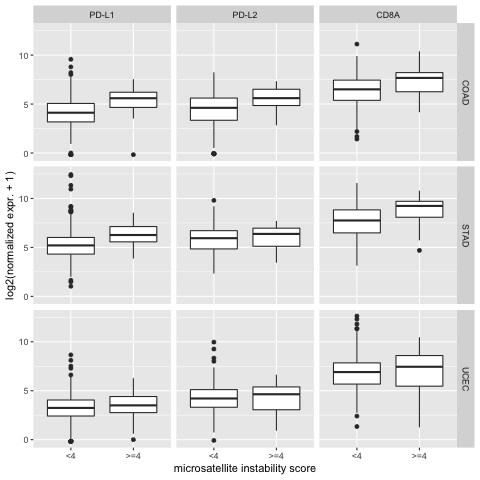
\includegraphics[height=8.0cm]{microsatpan2.png}
\caption{Top: Code for base graphics display of boxplot
corresponding to top left panel of lower display.
Bottom: Reassessment of immune infiltrate expression
patterns stratified by microsatellite instability
status and tumor type, as reported in \cite{Bailey2018}.
Figure \ref{compl} provides all
code needed to produce the nine panel display.}
\label{pancanPanel}
\end{figure}

